%! Author = borisdeletic
%! Date = 03/05/2023

% Preamble
\documentclass[11pt]{article}
\usepackage{algpseudocode}


% Document
\begin{document}

\section{Constrained Hamiltonian Monte Carlo}\label{sec:chmc}
    Consider the constrained distribution subject to the hard likelihood constraint
    \begin{equation}\label{eq:constrained_prior}
        \tilde{\pi}(\theta) = \begin{cases}
                                  \pi(\theta), & \mathcal{L}(\theta) > \mathcal{L}_0 \\
                                  0, & \text{otherwise}
                              \end{cases}
    \end{equation}
    Hamiltonian Monte Carlo can be modified to sample from a constrained prior, making it a viable
    technique for generating new live points in nested sampling.
    As described conceptually by Skilling~\cite{GMC} \& Betancourt~\cite{Betancourt_NS_CHMC}, reflecting
    off the iso-likelihood contours ensures that proposed samples are within the constrained distribution.
    When the next position $\theta_t$ in the trajectory would be below the likelihood constraint, we reflect the
    momentum off the boundary with normal $\mathbf{n} = - \nabla \log{\mathcal{L}(\theta)}$ as
    \begin{equation}\label{eq:reflection}
    \begin{aligned}
        \mathbf{n_R} &= M^{-1} \mathbf{n}, \\
        \mathbf{p'} &= \mathbf{p} - 2 \frac{ \mathbf{p} \cdot \mathbf{n_R} }{\mathbf{n} \cdot \mathbf{n_R}}. \mathbf{n}
    \end{aligned}
    \end{equation}

    \begin{figure}[h!]
        \centering
        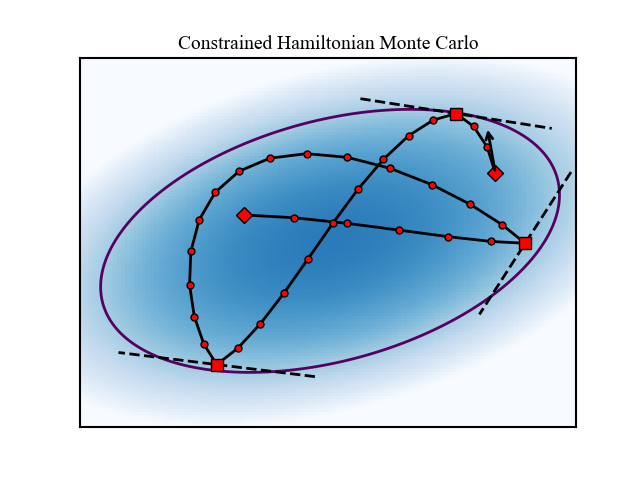
\includegraphics[width=\linewidth]{../figures/ConstrainedHMC}
        \caption{
            Hamiltonian Monte Carlo modified to reflect off iso-likelihood boundary $\mathcal{L}_0$.
            Initial point with randomly sampled momentum (diamond) moving through constrained prior
            distribution, $\tilde{\pi}(\theta)$, shown in blue.
            Finite step size $\epsilon$, shows discretisation of integrator with intermediate points (circles).
            Points which reflect off boundary (squares) do not fall exactly on the boundary due to discretization.
            After a fixed number of integration steps $L$, we propose a new sample from the constrained distribtion (diamond).
        }\label{fig:constrainedhmc}
    \end{figure}

    This sampling method can now be used for nested sampling, by using the point with the lowest
    likelihood at iteration $i$ with likelihood $\mathcal{L}_i$ to seed the generation of the next sample subject to
    the constraint $\mathcal{L} > \mathcal{L}_i$.

    Implementing this algorithm in practice poses new challenges with discretization, clustering, and parameter adaption.
    We propose a novel set of additional algorithms which are essential for a working implementation of
    Constrained HMC (CHMC).

\subsection{Epsilon Halving}\label{subsec:epsilon_halving}
    When performing reflections with a finite step size $\epsilon$, there is no guarantee that after a reflection,
    the next position will be within the constrained boundary.
    While this scenario is uncommon for smooth boundaries, over many iterations it is likely that at one time,
    no valid reflection will be found, causing the algorithm to crash.

    \begin{figure}[h!]
        \center
        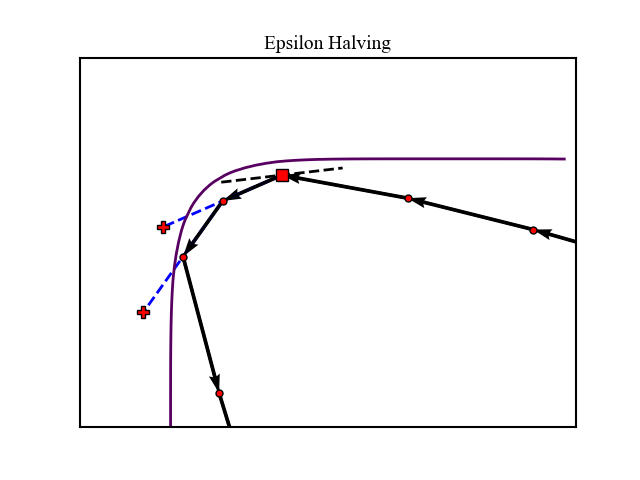
\includegraphics[width=\linewidth]{../figures/EpsilonHalving}
        \caption{
        For sharply curved boundaries, it is possible for the position after reflection (plus) to also lie outside the boundary
        constraint, leaving no valid reflections.
        In order for the algorithm to continue, a temporary step size is used to calculate the next position only.
        We iterate $\epsilon' = \epsilon / 2$ until the next point lies within the constraint.
        After a position within the constraint is found, we return back to integrating with $\epsilon_0$.
        }\label{fig:epsilon_halving}
    \end{figure}

    We propose a new reflection scheme which guarantees that a valid reflection will always be found, allowing the
    algorithm to continue.
    After a reflection, the next point is checked to see if it lies outside the boundary.
    If so, a temporary step size $\epsilon' = \epsilon / 2$ is used to re-integrate the position of the next point.
    Epsilon is repeatedly halved until a position within the boundary is found.
    This is guaranteed to produce a valid position in the limit $\epsilon' \rightarrow 0$ as a continuous reflection
    is performed.
    The algorithm then continues with the original $\epsilon_0$. \\

    \begin{algorithm}
        \caption{Epsilon Halving}
        \label{alg:epsilon_halving}
        \begin{algorithmic}
            \STATE \COMMENT{Momentum reflection}
            \STATE $\mathbf{p} \gets \mathbf{p} - 2 \left(\mathbf{p} \cdot \hat{ \mathbf{n} } \right) \hat{ \mathbf{n} }$
            \STATE
            \STATE $ \theta_{new} \gets \theta + \epsilon_0 \mathbf{p}$
            \STATE $ \epsilon' \gets \epsilon_0$
            \STATE
            \WHILE{ $\mathcal{L}(\theta_{new}) < \mathcal{L}_0$ }
                \STATE $\epsilon' \gets \epsilon' / 2$
                \STATE $ \theta_{new} \gets \theta + \epsilon' \mathbf{p}$
            \ENDWHILE
            \STATE
            \STATE $\theta \gets \theta_{new}$
        \end{algorithmic}
    \end{algorithm}


\subsection{Ergodicity}\label{subsec:ergodicity}
    Ergodicity and detailed balance are well known to be requirements of any MCMC algorithm~\cite{Metropolis_OG}.
    In practice however, no algorithm is truly ergodic due to imperfections in computation such as floating-point
    errors and the cyclic nature of pseudo-random number generators.
    The question then becomes whether the algorithm is \emph{sufficiently ergodic}.
    It is clear the process introduced by epsilon halving is not ergodic, therefore it is essential we ask
    whether our algorithm will maintain sufficient ergodicity.

    Adaptive techniques in MCMC methods have been shown to still converge to the required
    distribution~\cite{MCMC_Ergodicity}.
    Therefore, we argue that so long as our non-ergodic techniques are used infrequently, CHMC will be sufficiently
    ergodic to pass all statistical tests.

\subsection{Clustering}\label{subsec:clustering}

    Multi-modal posteriors pose a challenging problem for many MCMC sampling algorithms, with topological freezing
    causing significant complications~\cite{mangoubi2018_HMC_Multimodal}.
    In theory, nested sampling solves multi-modal distributions just as easily as uni-modal ones, hence
    its appeal as a tool for Bayesian inference.
    It is still important to carefully consider the sampling method used, to ensure that they do not
    cause a systematic bias.

    For instance, if there are not enough live points to cover the geometric features of the likelihood, it is
    possible for modes to `die out' and be missed by nested sampling.
    One solution is to use special measures to identify clusters of live points and treat them separately,
    as explored by \textsc{PolyChord} which uses a k-means algorithm for this purpose~\cite{Handley_polychord}.

    We illustrate how CHMC naturally solves clustering in multimodal distributions.
    Once the likelihood constraint is increased to the point where the contour splits into isolated volumes,
    all live points in the separate modes evolve completely independently of each other.

    \begin{figure}[h!]
        \center
        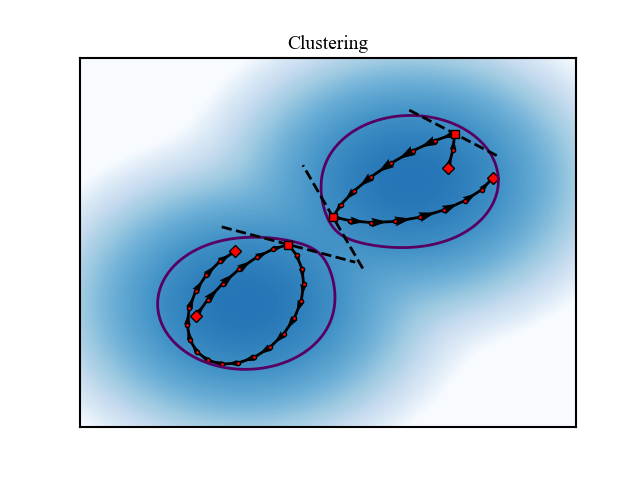
\includegraphics[width=\linewidth]{../figures/Clustering}
        \caption{
        Clustering in multi-modal distributions. When the iso-likelihood contour splits into
        two isolated modes, new samples generated are prevented from mixing with each other.
        The position $\mathbf{\theta}$ is restricted to stay within the posterior region contained by the volume,
        with no mechanism to cross into the other mode.
        }\label{fig:clustering}
    \end{figure}

\subsection{Topological Traps}\label{subsec:topological_trap}
    The natural clustering advantage of CHMC also brings rise a susceptibility to topological traps.
    Any live points in a local maxima will be forced to stay there, becoming further and further compressed until there
    is no more space new samples to be generated.

    We propose a new mechanism for sampling through topological traps based on \emph{reflection rate}.
    Define the reflection rate for live point $i$ as
    \begin{equation}\label{eq:reflect_rate}
        \mathcal{R}_i = \frac{r_i}{L},
    \end{equation}
    where $r_i$ is the number of reflections in the CHMC evolution.
    The motivation is that as we repeatedly resample points in an ever more constrained local maximum,
    $\mathcal{R}$ will approach 1 for these live points as they run out of room.

    We introduce a novel mechanism to move newly seeded live points from one mode into
    another, thereby allowing points to move from local to global maxima.

    \begin{algorithm}
        \caption{Nested sampling through topological traps using reflection rate}
        \label{alg:reflection_rate}
        \begin{algorithmic}
            \VARIABLES
            \STATE $\mathcal{R}_0$, Reflection rate threshold
            \STATE $\theta_r$, Parameters for a random live point
            \ENDVARIABLES
            \STATE
            \STATE $\theta_i$, Parameters for live point with lowest likelihood at iteration i
            \IF{ $\mathcal{R}(\theta_i) < \mathcal{R}_0$ }
            \STATE $\theta_{i+1} \gets$ \text{CHMC}($\theta_i$)
            \ELSE
            \STATE $\theta_{i+1} \gets$ \text{CHMC}($\theta_r$)
            \ENDIF
            \STATE Move $\theta_i$ to dead points
        \end{algorithmic}
    \end{algorithm}

    If the lowest likelihood live point has a reflection rate above some threshold, $\mathcal{R}_0$, we use a
    random live point as the seed for the next live point, instead of the current lowest likelihood live point.
    This ensures that given at least one live point is in the global maximum, eventually all the new live points will move
    into this mode where there is more `space`.

\end{document}